%!TEX root = lec16.tex
% ================================================================================
% Lecture 16, Slide 11
% ================================================================================
\begin{frame}[t]
  \mytitle{Step 3: Training --- Next Token Prediction}

\begin{columns}[T,totalwidth=\textwidth]

% ------------------------------------------------------------
\begin{column}[T]{0.50\textwidth}
\footnotesize
\vspace{4mm}

\textbf{\textcolor{blue}{Training objective}}

\vspace{2mm}
\begin{itemize}
  \item show text to the model
  \item hide the next token
  \item train it to predict the hidden token
\end{itemize}

\vspace{3mm}
\textbf{\textcolor{red}{Result:}}
\quad the model learns grammar, style, facts, and reasoning patterns
\y{as an emergent capability}.

\vspace{3mm}
{\tiny
Important: training is expensive \\
(compute + data).  \\
Using a model is cheap (inference).
}

\end{column}

% ------------------------------------------------------------
\begin{column}[T]{0.46\textwidth}
\footnotesize
\vspace{4mm}

\textbf{\textcolor{violet}{Why it can fail}}

\vspace{2mm}
\begin{itemize}
  \item it predicts \textbf{plausible text}
  \item not guaranteed truth
  \item can \textbf{hallucinate} details
\end{itemize}

\vspace{3mm}
{\tiny \textcolor{gray}{
Therefore: verification + grounding are crucial in professional use.
}}
\end{column}

\end{columns}

% ------------------------------------------------------------
% Next token prediction visualization (TikZ)
% ------------------------------------------------------------
\vspace{-11mm}
\hspace*{4cm}
\scalebox{0.70}{
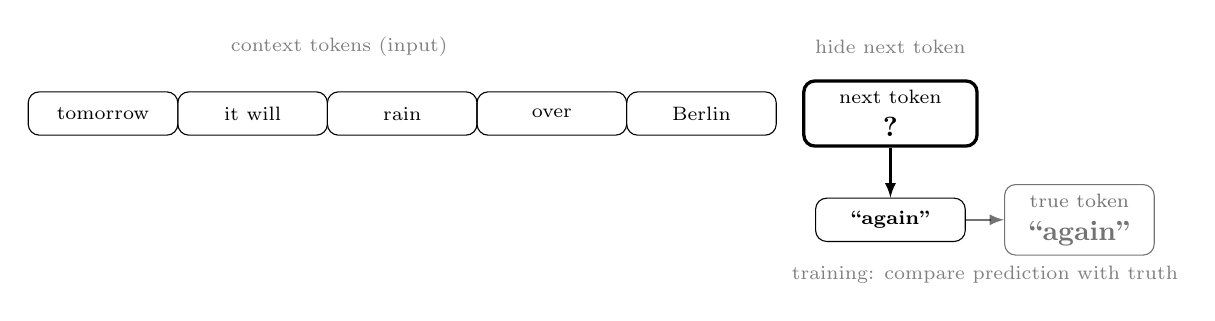
\begin{tikzpicture}[>=latex, x=1cm, y=1cm]

\tikzstyle{tok}=[draw, rounded corners, minimum width=1.9cm, minimum height=0.55cm, align=center]
\tikzstyle{tokfaint}=[draw, rounded corners, minimum width=1.9cm, minimum height=0.55cm, align=center, opacity=0.55]
\tikzstyle{tokspecial}=[draw, rounded corners, minimum width=2.2cm, minimum height=0.62cm, align=center, very thick]
\tikzstyle{arrow}=[->, thick]

% --- input tokens ---
\node[tok] (t1) at (-5.7,0) {\scriptsize tomorrow};
\node[tok] (t2) at (-3.8,0) {\scriptsize it will};
\node[tok] (t3) at (-1.9,0) {\scriptsize rain};
\node[tok] (t4) at ( 0.0,0) {\scriptsize over};
\node[tok] (t5) at ( 1.9,0) {\scriptsize Berlin};

% --- hidden next token ---
\node[tokspecial] (q) at (4.3,0) {\scriptsize next token\\\textbf{?}};

% --- model prediction ---
\node[tok] (pred) at (4.3,-1.35) {\scriptsize \textbf{``again''}};
\draw[arrow] (q.south) -- (pred.north);

% --- loss / training signal ---
\node[tokfaint] (true) at (6.7,-1.35) {\scriptsize true token\\\textbf{``again''}};
\draw[arrow, opacity=0.55] (pred.east) -- (true.west);

% --- captions ---
\node[align=center] at (-2.7,0.85) {\scriptsize \textcolor{gray}{context tokens (input)}};
\node[align=center] at (4.3,0.85) {\scriptsize \textcolor{gray}{hide next token}};
\node[align=center] at (5.5,-2.05) {\scriptsize \textcolor{gray}{training: compare prediction with truth}};

\end{tikzpicture}
}

\end{frame}
